% class
\documentclass[english]{scrartcl}


% text input and font
\usepackage[utf8]{inputenc}  % input in UTF-8
\usepackage[T1]{fontenc}  % output in T1 fonts (west European encoding)
\usepackage{lmodern}  % Latin modern font
\usepackage{babel}  % language package
\usepackage{amsmath, amssymb, amstext, mathtools}  % math packages (American Math Society) + correction of amsmath (mathtools) [loads amsmath automatically]
\usepackage{physics}  % macros for easier typesetting of physical formulas
\usepackage{letltxmacro}  % \let command for robust macros (new sqrt)


% page geometry
\usepackage{scrlayer-scrpage}  % page formatting with KOMA options
\usepackage[paper=a4paper, hmargin=3cm, vmargin=2.5cm, includehead, includefoot]{geometry}


% floats
\usepackage[hypcap=false, labelfont=bf]{caption, subcaption}  % caption editing - hypcap warning with hyperref
\usepackage{float}  % for [H] (forced here) specifier
\usepackage{tabularray}
\usepackage{diagbox}  % table cells with diagonal lines


% graphical input
\usepackage{graphicx}  % input JPEG, PNG, PDF, etc.
\usepackage{pdfpages}  % input PDF as whole pages
\usepackage{lastpage}  % reference to last page


% text
\usepackage[locale=DE, uncertainty-mode=separate]{siunitx}  % SI units, German formatting - \pm stays \pm instead of ..(.)
\usepackage{icomma}  % no space after commas instead of English points) in decimal values
\usepackage{enumitem}  % better enumerating with style options
\usepackage{nicefrac}  % inline-fractions in n/d-style
\usepackage{fancyvrb}  % Verbatim environment with better options (capital V!)

% literacy
\usepackage[style=apa]{biblatex}  % backend=Biber is standard
\usepackage{csquotes}  % better quotation - should also be used in combination with package babel (warning)
\usepackage{xurl}  % breaks links - after BibLaTeX, but before hyperref!
\usepackage[hidelinks]{hyperref}  % produces most errors, last to load


% KOMA setups
% header and footer
\pagestyle{scrheadings}  % KOMA style
\clearpairofpagestyles  % reset
\setkomafont{pageheadfoot}{\normalfont}  % standard font in header and footer
\setlength{\headheight}{27.2pt}  % just look at the warning
\ihead{DA II\\Assignment 4}  % inner (left) head
\chead{\textsc{Wachmann} Elias (12004232)}  % center head
\ohead{\today}  % outer (right) head
\cfoot{\pagemark{} / \pageref*{LastPage}}  % center foot - *: ref but no hyperlink
% {}: empty statement
% \ : protected space
% \,: small space
\DeclareTOCStyleEntry{dottedtocline}{section}  % sections in TableOfContents with dotted lines
\KOMAoptions{parskip=half-}  % paragraphs with half a line height space instead of indentation, last line with no special treatment


% package setups

% BibLaTeX source
% \addbibresource{halbleiterdiode.bib}


% rewrite names (babel overwrites German with standard English names, therefore at document beginn [after everything is loaded])
% \AtBeginDocument{\renewcommand{\refname}{Literaturverzeichnis}}
% others:
% \contentsname
% \listtablename
% \listfigurename


% new sqrt
% https://en.wikibooks.org/wiki/LaTeX/Mathematics
\makeatletter
\let\oldr@@t\r@@t
\def\r@@t#1#2{%
\setbox0=\hbox{$\oldr@@t#1{#2\,}$}\dimen0=\ht0
\advance\dimen0-0.2\ht0
\setbox2=\hbox{\vrule height\ht0 depth -\dimen0}%
{\box0\lower0.4pt\box2}}
\LetLtxMacro{\oldsqrt}{\sqrt}
\renewcommand*{\sqrt}[2][\ ]{\oldsqrt[#1]{#2} }
\makeatother

 
% tabularray
% imports_and_setups{
%     expl3,
%     xparse,
%     ninecolors
%     \hypersetup{pdfborder={0 0 0}}
% }
\RequirePackage{tabularray}  % like \usepackage but for packages
\UseTblrLibrary{siunitx}  % siunitx suited for tabularray
% TRIPLE BRACKETS {{{}}} to protect strings from \num{} interpretation in S columns
\UseTblrLibrary{diagbox}  % diagbox suited for tabularray
\UseTblrLibrary{varwidth}  % measure cell width using package 'varwidth'

% standard environment
\SetTblrInner{
    hlines,
    vlines,
    columns={
            halign=c,
            valign=m,
        },
    measure=vbox,
}

% X columns
\NewTblrEnviron{tblrx}
\SetTblrInner[tblrx]{
    hlines,
    vlines,
    columns={
            halign=c,
            valign=m,
            co=1,  % coefficient of width for expendable columns (X columns)
        },
    width=\linewidth,
    vspan=minimal,
    measure=vbox,
}

% -X columns
\NewTblrEnviron{tblr-x}
\SetTblrInner[tblr-x]{
    hlines,
    vlines,
    columns={
            halign=c,
            valign=m,
            co=-1,  % shrinks X column down to natural width
        },
    width=\linewidth,
    vspan=minimal,
    measure=vbox,
}

% no hline and vline left and on top of first cell
\NewTblrEnviron{tblr_omit_first_cell}
\SetTblrInner[tblr_omit_first_cell]{
    hlines,
    vlines,
    columns={
            halign=c,
            valign=m,
        },
    hspan=even,
    vspan=minimal,
    %
    hline{1}={1}{white},  % first row, only first cell
    vline{1}={1}{white},
    measure=vbox,
}

\usepackage{pythonhighlight}
\usepackage{amsmath}
\usepackage{algorithm}
\usepackage[noend]{algpseudocode}

% individual settings
%\addbibresource{beschreibung.bib}  % database import with absolute path - file ending!
\newcommand{\code}{\texttt}



\begin{document}
\begin{titlepage}
    \begin{center}
        \vspace{1cm}
        \Huge
        \textbf{Data Structures and Algorithms II}
        \vspace{5mm}

        \Large
        Assignment 4
        \vspace{5mm}


        \textbf{Wachmann Elias}


        \today
    \end{center}
\end{titlepage}

\clearpage
% \tableofcontents
\newpage

\section{Task Description}
\label{sec:problem}
\textbf{Triangulation 3-coloring} 
\newline
Your are given a triangulation of a point set. Your task is to design an efficient algorithm that constructs a valid 3-coloring of the points of the triangulation or determines that such a 3-coloring does not exist. A 3-coloring of the points is valid if any two points that are connected with an edge have different colors.
The n points of the triangulation are labeled with the integers $\{1, \dots, n\}$. The triangulation is given by a list of edges with additional triangle points (see Figure 1 for an example):
\begin{itemize}
    \item Every edge is given by the labels of its two end points (first the smaller point label, then the larger one).
    \item For every edge, the labels of the point(s) with which the edge forms a triangle (a bounded triangular face) in the triangulation is given (two labels for interior edges and one label for edges on the boundary of the convex hull).
\end{itemize}
\begin{figure}[H]
    \centering
    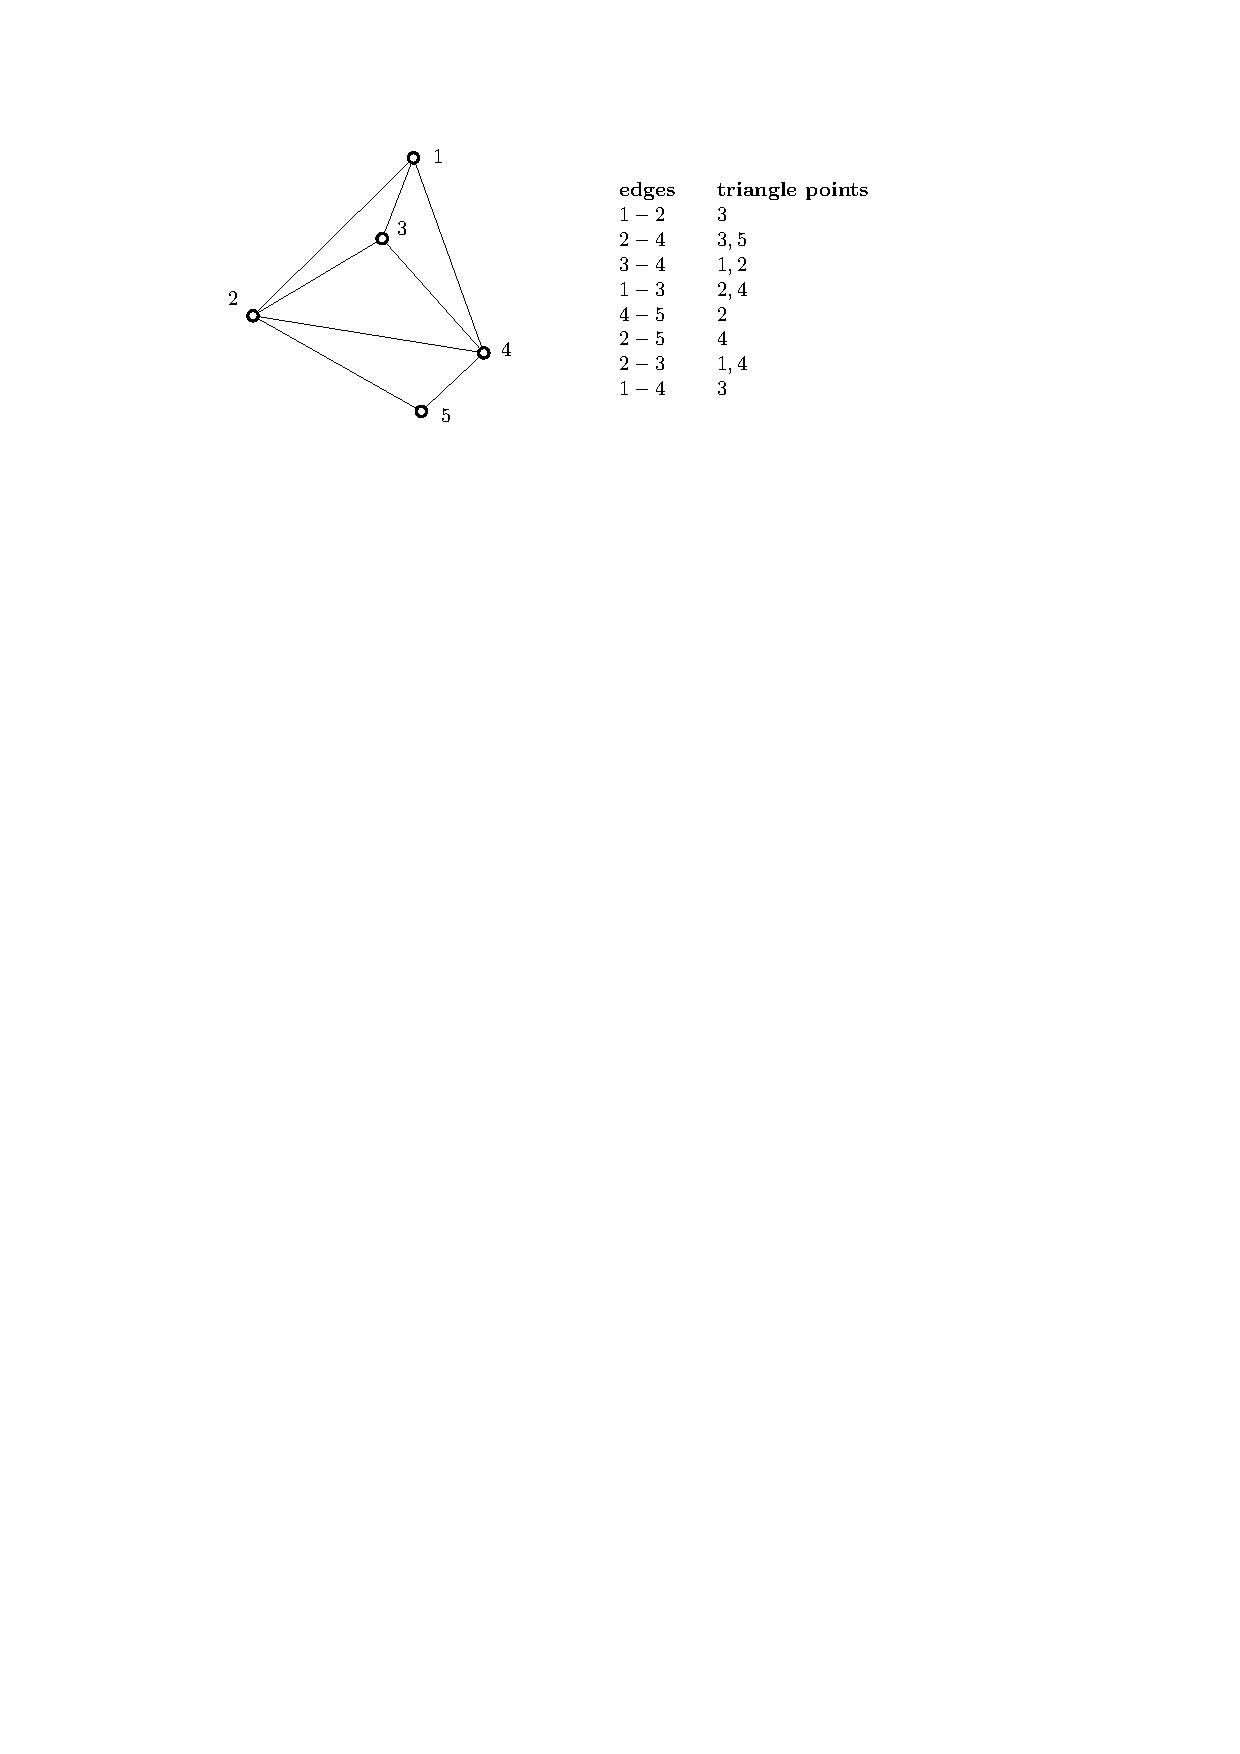
\includegraphics{img/plain.pdf}
    \caption{Example of a triangulation and a list of its edges with triangle points.}
    \label{fig:fig1}
\end{figure}
Explain and describe your algorithm in detail, analyze its runtime and memory requirements, and give reasons for the correctness of your solution.

\section{Description of algorithm}
\label{sec:description}
\textbf{Note}: It is assumed from the example, that the edges are always given with the lower vertex number in the first place e.g. 1-5 instead of 5-1. If this is not a given, the edge representation could be changed to conform to the above constraint in linear time, thus not increasing the asymptotic runtime. 
\\ \\
\textbf{General}: The algorithm takes a list of edges with additional triangle points \code{EDGES} (as described above) as input and outputs a 3-coloring of the graph \code{COLORS} if it is possible. If no valid 3-coloring of the given graph exists, the algorithm exits and indicates that no such coloring is possible (\code{COLORS} is not returned in this case).
\\
The algorithm starts with the \textbf{Setup} step, then the Points on the first edge and it's triangle points are colored in \textbf{Start}, after which \textbf{Loop} takes care of the remaining Points. Afterwards the validity of the coloring is checked. 
\begin{enumerate}
    \item \textbf{Setup:}\\ First get number of Points. The Maximum is given, by the maximum (number) in triangle points. Use this number to create an array \code{COLORS} with this size for the colors of the vertices. Store edges (keys) and triangle points (values) in a hashmap \code{EDGE\_DIC} for fast access. Setup counter \code{counter} which tracks how many vertices need to be colored in. Setup empty queue \code{NEXTEDGES} for neighboring edges.
    \item \textbf{Start:}\\ An arbitrary start edge, for example the first in \code{EDGES} is chosen as \code{cur\_edge}. The two endpoints $p_1$ and $p_2$ of \code{cur\_edge} are colored with $c_1$ and $c_2$ respectively. Then the triangle points are colored \footnote{Depending on the edge type either one (outer edge e.g. 1-2 in \autoref{fig:fig1}) or a maximum of two triangle points (inner edge e.g. 1-3 in \autoref{fig:fig1}) are colored in.} in. Finally the \code{counter} is decreased by the number of vertices which were colored in and \code{cur\_edge} is deleted from \code{EDGE\_DIC}.  
    \item \textbf{Loop:} The Loop is executed while \code{counter} is not 0. \\ All neighbors of \code{cur\_edge} which were not visited before (meaning they were never \code{cur\_edge}) are added to the queue \code{NEXTEDGES}. Neighbors to the \code{cur\_edge} are edges which form a triangle with the \code{cur\_edge} if the two endpoints of the so given path are connected. 
    \footnote{This definition of neighbors guarantees that the so formed triangle already has two colored points, thus making the coloring of the third trivial. \\ \textbf{Example:} The edge 1-2 in \autoref{fig:fig1} has 2 neighbors (1-3 and 2-3) according to the above definition, whereas an inner edge has 4: e.g. 3-4 has 1-3, 1-4, 2-3 and 2-4 as neighbors} 
    Now \code{cur\_edge} is set to the last edge in \code{NEXTEDGES} (according to the FIFO-principle). %fix vielleicht argumentieren warum das nie leer sein kann.
    The colors $c_1$ and $c_2$ of $p_1$ and $p_2$ of \code{cur\_edge} are checked. If they are the same, algorithm terminates because no valid 3-coloring of the given graph exists. Otherwise the algorithm tries to color the triangle points of \code{cur\_edge} (at least one [outer edge] and at most 2 triangle points for inner edges). If the triangle point is already colored with $c_3$, it is check if the color is neither $c_1$ nor $c_2$, if the color would match either $c_1$ or $c_2$ the algorithm terminates as in the aforementioned case $c_1$ equals $c_2$. If the the triangle point is properly colored nothing happens and if applicable the second triangle point is checked. In the case that the triangle point isn't colored already, it is colored with $c_3$ such that $c_3$ is different than $c_2$ and $c_1$. Finally the \code{counter} is decreased by the number of vertices which were colored in and \code{cur\_edge} is deleted from \code{EDGE\_DIC}. $\rightarrow$ Loop
    \item \textbf{Check validity of coloring of remaining edges:}\\For the graph in \autoref{fig:fig1} \textbf{without Point 5} (without edges 2-5 and 4-5) the algorithm could produce a impossible coloring and end. \footnote{The \code{counter} would reach 0 if the start edge would be 1-3 (The loop would be skipped and thus no checks would be done)} To avoid these edge cases one could check all edges and their triangle points for matching colors as described in \enquote*{Loop} above. However color-checking only the remaining edge-triangle-point-pairs in \code{EDGE\_DIC} is sufficient, because these are the edges which were never \code{cur\_edge}. Asymptotically this reduction in remaining edge-triangle-point-pair color checks doesn't matter as we'll see below. 
\end{enumerate}


\section{Space complexity / memory requirements}
\label{sec:space_compl}
\textbf{Note:} As derived from Euler's formula in the lecture for a connected, simple, planar graph the following holds true for $v \geq 3$:
\begin{equation}
    \label{eq:euler}
    e \leq 3 v-6 
\end{equation}
Where $e$ is the number of edges, and $v$ the number of vertices in the graph. For this reason asymptotically the number of edges as well as the number of vertices are the same ($\mathcal{O}(e) = \mathcal{O}(v)$). 
For this reason the analysis in the current section, as well as \autoref{sec:runtime_comp} will use the size of the input, more precisely the number of edges $n$ in \code{EDGES}.\\
\newline
The memory requirements of the algorithm is given as follows:
\begin{itemize}
    \item \code{EDGES} [input] stores all $n$ edges of the graph which results in $\mathcal{O}(n)$ space complexity.
    \item \code{COLORS} [output] stores asymptotically (as shown above) $\mathcal{O}(n)$ colors of the vertices which results in $\mathcal{O}(n)$ space complexity
    \item \code{EDGE\_DIC} stores all the edges from the [input] \code{EDGES} as key-value pair in a hashmap which requires $\mathcal{O}(n)$ space. 
    \item \code{NEXTEDGES} stores at most $n-1$ edges \footnote{$n-1$ is for example true in the trivial case with $n=3$} which results in $\mathcal{O}(n)$ space complexity.
    \item Local variables: \code{counter} and \code{cur\_edge} have $\mathcal{O}(1)$ space complexity.
\end{itemize}
All together the data structures require $\mathcal{O}(n)$ space. 

\section{Runtime complexity}
\label{sec:runtime_comp}
The runtime complexity analysis is based on the number of edges $n$ in the input \code{EDGES}. As shown above in \autoref{eq:euler} $n$, being the number of edges, is asymptotically the same as $v$ the number of vertices.\\
The Analysis is split into the same four parts as in \autoref{sec:description}:
\begin{enumerate}
    \item \textbf{Setup:} 
\end{enumerate}
\section{Correctness of the algorithm}
\label{sec:correctness}
\textbf{TODO}




\clearpage
% % Literaturverzeichnis
% \printbibliography

% % Abbildungsverzeichnis
% \listoffigures

% % Tabellenverzeichnis
% \listoftables

\end{document}
